\section{Results}
\label{sec:results}

We report five findings, in the order the framework implies: coverage exists
(R1), selectors mostly fail to convert it (R2--R3), compute-matching removes
most of what remains (R4), and the two cheap diagnostics predict all of this in
advance (R5).

\begin{figure}[t]
\centering
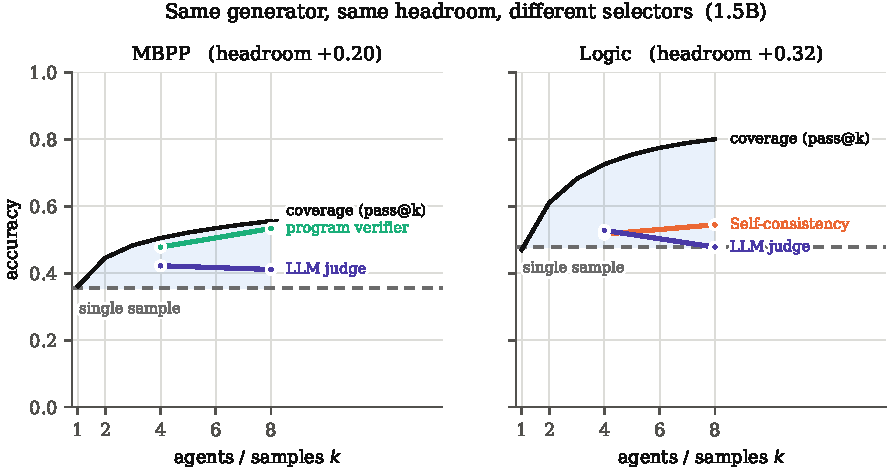
\includegraphics[width=\textwidth]{figures/fig1_thesis.pdf}
\caption{The decomposition on a high- and a low-asymmetry family. The shaded
band is coverage headroom---accuracy that already exists in the candidate
pool. Where a selector's curve sits inside that band is its selection
efficiency $\eff$. The two panels share a generator and differ only in how
checkable the task is.}
\label{fig:thesis}
\end{figure}

\subsection{R1: Coverage headroom is large and nearly universal}

\begin{figure}[t]
\centering
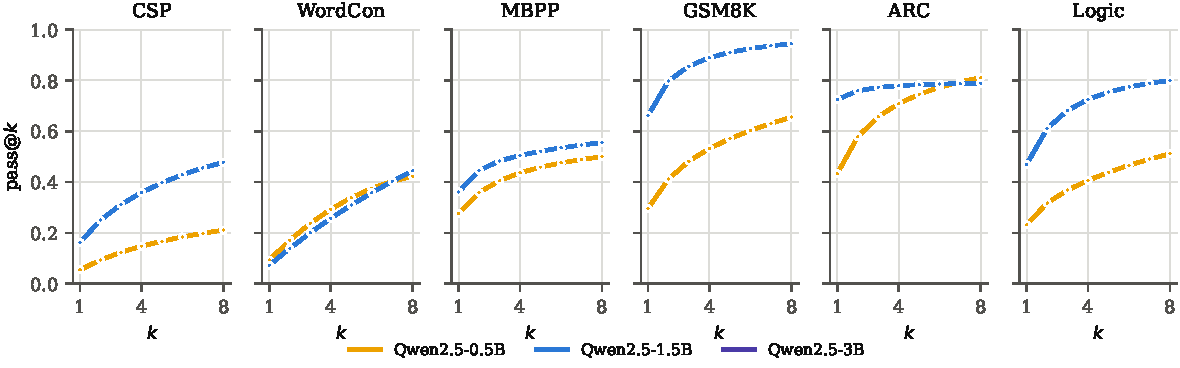
\includegraphics[width=\textwidth]{figures/fig2_coverage.pdf}
\caption{Unbiased $\mathrm{pass}@k$ by family and model. Headroom---the gap
between $k=1$ and $k=8$---is substantial almost everywhere, so the coverage
factor is rarely what limits a multi-agent system.}
\label{fig:coverage}
\end{figure}

Figure~\ref{fig:coverage} shows $\mathrm{pass}@k$ for every family and model.
Consistent with the repeated-sampling literature
\citep{brown2024monkeys,snell2024scaling}, coverage rises steeply with $k$:
sampling eight times rather than once adds substantial headroom in nearly every
cell. Table~\ref{tab:main} gives the corresponding single-sample accuracies.

The practical reading is that the first factor of
Equation~\eqref{eq:decomp-intro} is usually \emph{not} the binding constraint.
Multi-agent systems fail, when they fail, on the second factor.

\begin{table}[t]
\centering\small
\begin{tabular}{lrrrrrr}
\toprule
Architecture & CSP & WordCon & MBPP & GSM8K & ARC & Logic \\
\midrule
Single sample & 0.21 & 0.10 & 0.36 & 0.64 & 0.70 & 0.48 \\
Sequential refine & 0.34 & 0.03 & 0.39 & 0.67 & 0.64 & 0.40 \\
Self-consistency & 0.23 & -- & -- & 0.87 & 0.71 & 0.54 \\
Ensemble + LLM judge & 0.20 & 0.07 & 0.41 & 0.69 & 0.70 & 0.48 \\
Ensemble + program verifier & 0.48 & 0.44 & 0.53 & -- & -- & -- \\
Debate (3$\times$2) & 0.19 & 0.02 & 0.38 & 0.53 & 0.72 & 0.53 \\
\midrule
\textit{Ensemble + oracle} (ceiling) & 0.48 & 0.44 & 0.56 & 0.94 & 0.79 & 0.80 \\
\midrule
\multicolumn{7}{l}{\textit{mean tokens per task}} \\
\quad Single sample & 366 & 78 & 125 & 309 & 101 & 81 \\
\quad Sequential refine & 2,274 & 449 & 908 & 1,709 & 762 & 929 \\
\quad Ensemble + LLM judge & 5,012 & 849 & 1,454 & 4,052 & 1,028 & 961 \\
\quad Debate (3$\times$2) & 2,532 & 637 & 1,093 & 2,194 & 736 & 662 \\
\bottomrule
\end{tabular}
\caption{Accuracy by architecture and family, and mean token cost per task.
The oracle row is the coverage ceiling: it is not deployable, and the distance
between it and the deployable selectors is the accuracy the ensemble generated
but could not identify.}
\label{tab:main}
\end{table}

\subsection{R2: The generator--verifier gap varies enormously, and is sometimes negative}

\begin{table}[t]
\centering\small
\begin{tabular}{llrrrrrr}
\toprule
Model & Diagnostic & CSP & WordCon & MBPP & GSM8K & ARC & Logic \\
\midrule
Qwen2.5-0.5B & $\gap$ (verifier) & +0.00 & +0.00 & +0.00 & +0.00 & +0.00 & +0.00 \\
 & $\plur$ (plurality) & +0.03 & -- & -- & +0.13 & +0.03 & -0.07 \\
 & position bias & 1.00 & 0.00 & 0.20 & 1.00 & 1.00 & 1.00 \\
 & order consistency & 0.00 & 0.00 & 0.20 & 0.00 & 0.00 & 0.00 \\
\addlinespace
Qwen2.5-1.5B & $\gap$ (verifier) & +0.42 & -0.27 & +0.42 & +0.05 & +0.09 & +0.05 \\
 & $\plur$ (plurality) & +0.07 & -- & -- & +0.30 & +0.00 & +0.00 \\
 & position bias & 0.29 & 0.59 & 0.54 & 0.42 & 0.36 & 0.18 \\
 & order consistency & 0.58 & 0.45 & 0.58 & 0.65 & 0.00 & 0.16 \\
\addlinespace
\bottomrule
\end{tabular}
\caption{The two cheap diagnostics measured on the \nCalib{}-task calibration
split, with judge position bias (the rate at which the first-listed candidate
is chosen; $0.5$ is unbiased) and order consistency (how often the judge names
the same candidate when the two are presented in the opposite order; a judge
that simply picks a position scores $0$). $\gap$ ranges from \Gmin{} to \Gmax{};
\nGnegative{} cells are negative, meaning the model prefers its own incorrect
answers more often than its correct ones.}
\label{tab:diagnostics}
\end{table}

Table~\ref{tab:diagnostics} reports $\gap$ and $\plur$ per cell. The spread is
the central empirical fact of this paper: the same model, asked the same kind
of question---``which of these two answers is right?''---ranges from near-perfect
discrimination on families whose answers can be checked mechanically to
\emph{below chance} on families where checking means redoing the derivation.
\nGnegative{} of our cells have $\gap < 0$.

A negative gap deserves emphasis because it is not merely a small gain. It
means a model critic is an \emph{actively harmful} selector: it systematically
prefers wrong answers, so adding it to a pipeline reduces accuracy below
picking a candidate at random. Part of the mechanism is visible in the position
bias column, where the smallest model chooses the first-listed candidate up to
\maxPositionBias{} of the time, reproducing at small scale the bias documented
for stronger judges by \citet{zheng2023judge}. Order consistency falls as low
as \minOrderConsistency{}: on those cells the judge is not evaluating the
candidates at all, it is naming a position, and reversing the presentation
reverses its verdict.

Because a position-picking judge would otherwise inherit spurious
discrimination from any imbalance in which side happens to hold the correct
answer, every pair in our probe is presented twice, once in each order, and
$\gap$ averages over both. Under this counterbalancing a pure position-picker
scores exactly chance by construction. We flag this because our own first
implementation randomised the side independently per pair, which at
$n\approx20$ produced an apparent $\gap$ of $+0.40$ on a cell whose judge chose
the first option $100\%$ of the time.

\subsection{R3: Selection efficiency, not coverage, is what separates architectures}

\begin{figure}[t]
\centering
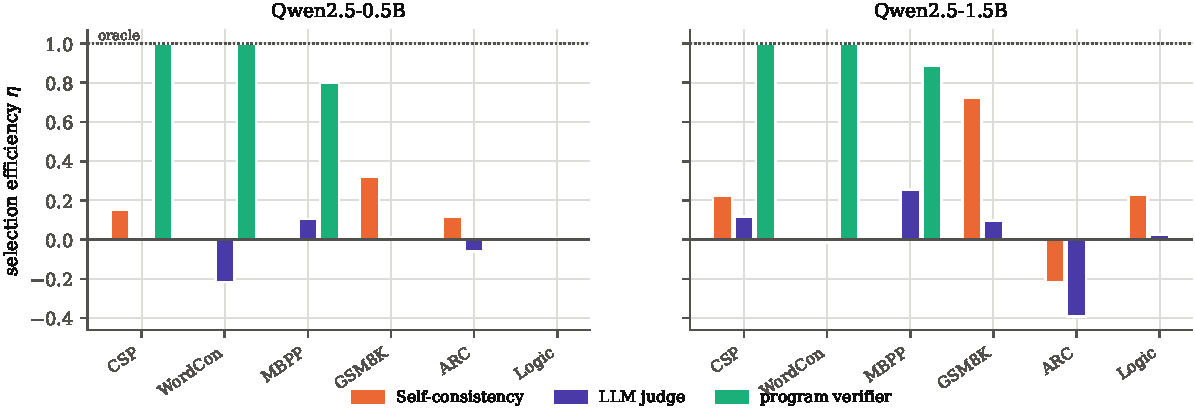
\includegraphics[width=\textwidth]{figures/fig3_eta.pdf}
\caption{Selection efficiency $\eff$ at $k=8$. A value of $1$ means the
selector captures all available headroom; $0$ means it does no better than
picking at random; negative means it does worse.}
\label{fig:eta}
\end{figure}

Figure~\ref{fig:eta} decomposes the architectures by $\eff$. Across
\nEtaCells{} measured cells the median program verifier attains
$\eff = \etaProgMedian{}$, the median self-consistency $\etaVoteMedian{}$, and
the median LLM judge $\etaJudgeMedian{}$, with a worst case of
$\etaJudgeMin{}$; \nEtaNegative{} cells are negative.

Two caveats keep this honest. First, for CSP and WordCon the program verifier
is a \emph{complete} checker---it tests exactly the property the grader
tests---so $\eff=1$ there is true by construction and demonstrates only that
the ceiling is attainable at zero token cost, not that verification is
magically easy. The informative case is MBPP, where the verifier sees one test
and grading uses held-out tests, so its efficiency is earned rather than
assumed. Second, self-consistency requires a canonical short answer and is
simply undefined for WordCon and MBPP; we report that rather than forcing a
degenerate clustering.

\subsection{R4: Token-matching removes most of the apparent benefit}

\begin{figure}[t]
\centering
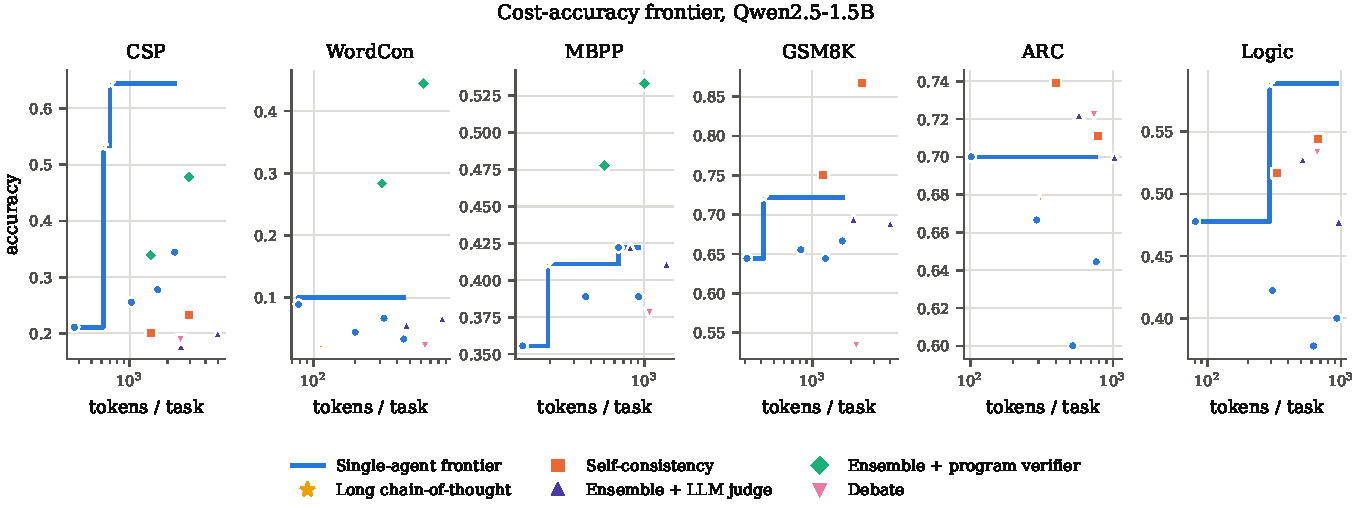
\includegraphics[width=\textwidth]{figures/fig4_frontier.pdf}
\caption{Accuracy against token cost. The line is the single-agent frontier:
the upper envelope of sequential refinement and long chain-of-thought at each
budget. A multi-agent point above the line earns its compute; a point below it
would have done better as one agent thinking longer.}
\label{fig:frontier}
\end{figure}

\begin{figure}[t]
\centering
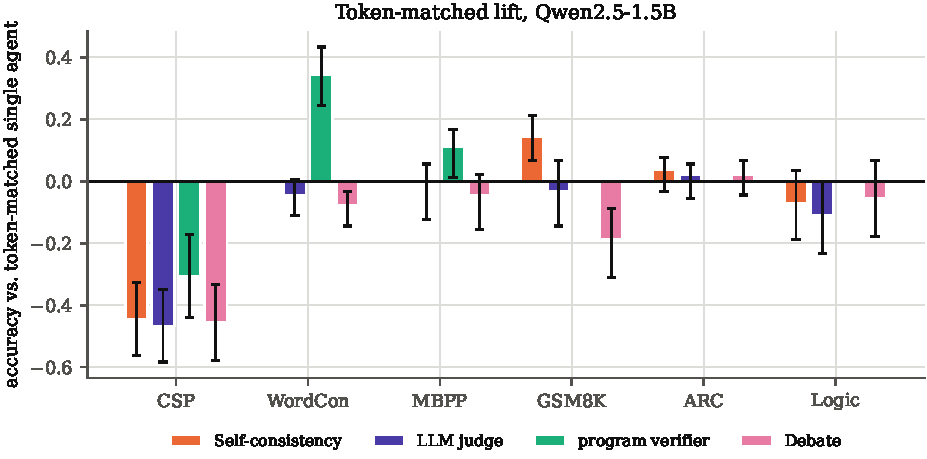
\includegraphics[width=0.82\textwidth]{figures/fig5_matched_lift.pdf}
\caption{Token-matched lift with $95\%$ cluster-bootstrap intervals, in which
both the multi-agent accuracy and the single-agent frontier are recomputed
inside every resample.}
\label{fig:matched}
\end{figure}

\begin{table}[t]
\centering\small
\begin{tabular}{lrrrr}
\toprule
Family & Self-consistency & LLM judge & program verifier & Debate (3$\times$2) \\
\midrule
CSP & $-0.444$$^{*}$ & $-0.467$$^{*}$ & $-0.306$$^{*}$ & $-0.456$$^{*}$ \\
WordCon & -- & $-0.044$ & $+0.344$$^{*}$ & $-0.078$ \\
MBPP & -- & $-0.011$ & $+0.111$$^{*}$ & $-0.044$ \\
GSM8K & $+0.144$$^{*}$ & $-0.033$ & -- & $-0.189$$^{*}$ \\
ARC & $+0.039$ & $+0.022$ & -- & $+0.022$ \\
Logic & $-0.072$ & $-0.111$ & -- & $-0.056$ \\
\bottomrule
\end{tabular}
\caption{Token-matched lift by family and architecture. $^{*}$ marks
Holm--Bonferroni adjusted $p<0.05$. Compare against the naive comparison
against a single sample, which is what most of the literature reports.}
\label{tab:matched}
\end{table}

This is the result with the most direct bearing on practice. Measured against a
single sample---the comparison most commonly reported---the median architecture
gains \medianNaiveLift{}. Measured against a single agent given the same token
budget, the median becomes \medianMatchedLift{}, and
\fracMatchedNegative{} of all configurations are net negative. Of the
\nCellsPositiveNaive{} cells that appear to benefit under the naive comparison,
\nCellsFlipped{} (\nFlip{}) do not survive compute-matching.

The architectures do not fail equally, and the pattern is the one the framework
predicts. Systems whose selector is an external program retain their advantage,
because their verification is both reliable and free. Systems whose selector is
the model judging itself lose most or all of theirs, because they pay $k$ times
the tokens for a selector whose $\gap$ does not support the choice. Debate is
the most expensive arm and among the weakest per token, which is consistent
with its gains being attributable to additional sampling rather than to the
exchange of arguments---the interpretation \citet{li2024moreagents} reach from
the opposite direction.

\subsection{R5: The diagnostics predict lift before the system is built}

\begin{figure}[t]
\centering
\begin{subfigure}{0.48\textwidth}
\centering
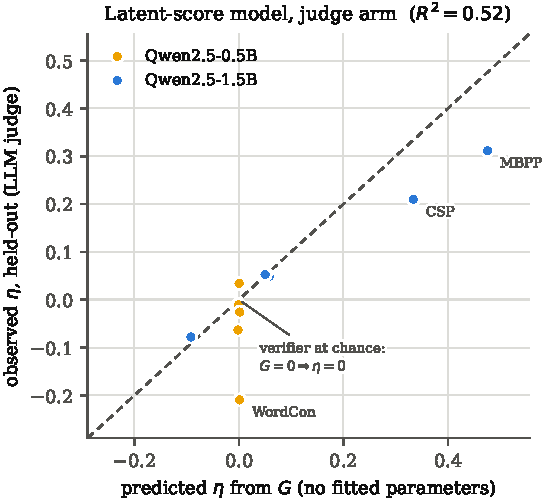
\includegraphics[width=\textwidth]{figures/fig8_theory.pdf}
\caption{Latent-score model: predicted versus observed $\eff$.}
\end{subfigure}\hfill
\begin{subfigure}{0.48\textwidth}
\centering
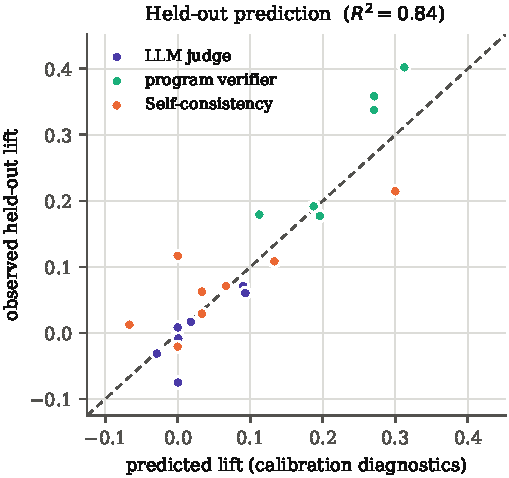
\includegraphics[width=\textwidth]{figures/fig6_prediction.pdf}
\caption{Held-out lift, predicted from calibration diagnostics.}
\end{subfigure}
\caption{Both panels compare against the identity line, not a fitted
regression: the theory predicts the \emph{value}, so a fitted slope would hide
bias.}
\label{fig:prediction}
\end{figure}

Finally we test whether the framework is usable prospectively. Features come
from the \nCalib{}-task calibration split only; targets come from the
\nTest{}-task held-out split; the split was fixed before any model ran.

A discriminating pair requires one correct and one incorrect candidate in the
same pool, so on families where accuracy is very low or very high, $\gap$ rests
on few comparisons. We therefore pre-specified a minimum of \minPairs{} scored
pairs for cells whose prediction depends on $\gap$, which excludes
\nDroppedLowPairs{} cells; without that filter the same analysis gives
$R^2 = \rTwoAprioriNoFilter{}$, so the conclusion does not rest on the choice.

Across \nPredCells{} cells, the a priori prediction---$\gap$ and $\plur$
measured on calibration, passed through Proposition~\ref{prop:latent}, with no
fitted parameters---attains $R^2 = \rTwoApriori{}$ against the identity line
(Pearson $r = \corrApriori{}$, mean absolute error \maeApriori{}). Simply transferring measured $\eff$ from calibration to held-out attains
$R^2 = \rTwoTransfer{}$, which upper-bounds what any diagnostic could achieve
given sampling noise; the a priori prediction essentially matches it, so the
cheap probe loses little against directly measuring the thing it estimates.

Restricted to the judge arm alone---where the latent-score model does all of
the work, rather than the coarse separation between verifier types---the
prediction attains $R^2 = \rTwoJudgeArm{}$ over \nJudgeArmCells{} cells
(Figure~\ref{fig:prediction}a). Two features of that panel are worth stating
plainly. Every cell with $\gap=0$ is predicted to have $\eff=0$ exactly, which
is not a fitted success but a property of the model; the observed values
scatter around zero as sampling noise. And at the high end the model
\emph{over}-predicts: the two cells with the largest gaps sit visibly below
the identity line. We take this as the expected cost of assuming
conditionally independent, equally dispersed scores---a listwise judge that
sees all candidates at once violates both---and we report it rather than
introducing a free parameter to absorb it.

Turned into the binary decision of Equation~\eqref{eq:rule}---build the ensemble,
or spend the tokens on one agent---the rule agrees with the token-matched
outcome in \decisionAgreement{} of \nDecisionCells{} cells, at precision
\decisionPrecision{} and recall \decisionRecall{}. We report that number
against the right yardstick rather than against chance: because multi-agent
architectures fail so often in our data, simply answering ``do not build'' every
time is already correct \decisionBaseline{} of the time, so the diagnostic buys
\decisionLift{} percentage points over that baseline. This is a real but modest
gain, and it is the weakest of our results. The continuous prediction is the
claim we would stand behind: the diagnostics estimate \emph{how much} an
architecture will gain far better than they resolve the knife-edge cases where
the gain is near zero, which is precisely where a binary rule is forced to
commit. A practitioner is better served by the predicted magnitude and its
uncertainty than by the rule's verdict.

That the majority baseline sits at \decisionBaseline{} is itself the finding
worth carrying away: across \nDecisionCells{} architecture--task pairs drawn
from the designs the literature recommends, the prior that multi-agent
structure will not survive compute-matching is correct more often than not.

\subsection{R6: How the diagnostics move with scale}

\begin{figure}[t]
\centering
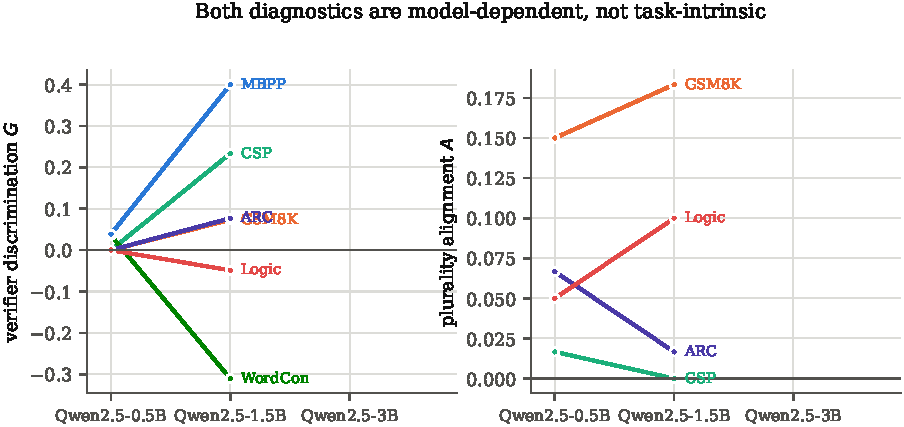
\includegraphics[width=0.85\textwidth]{figures/fig7_scale.pdf}
\caption{Both diagnostics across model scale. They are properties of a
(model, task) pair, not of the task alone, so they must be re-measured when
either changes.}
\label{fig:scale}
\end{figure}

Figure~\ref{fig:scale} contrasts $\gap$ and $\plur$ at 0.5B and 1.5B. The important
qualitative point is that neither is a property of the task alone: the same
family can move from a negative to a positive gap as the model grows, which
means a multi-agent design that fails at one scale may succeed at another and
vice versa. This is the mechanism we think underlies much of the disagreement in
the literature. We state explicitly what two points cannot do: they show the diagnostics are model-dependent, and they establish no trend and license no extrapolation. A third scale point is the single most valuable addition to this study, and the released code runs it unchanged.
